\documentclass[12pt]{article}
\usepackage[utf8]{inputenc}
\usepackage{float}
\usepackage{amsmath}

\usepackage[hmargin=3cm,vmargin=6.0cm]{geometry}
%\topmargin=0cm
\topmargin=-2cm
\addtolength{\textheight}{6.5cm}
\addtolength{\textwidth}{2.0cm}
%\setlength{\leftmargin}{-5cm}
\setlength{\oddsidemargin}{0.0cm}
\setlength{\evensidemargin}{0.0cm}

%misc libraries goes here
\usepackage{tikz}
\newcommand{\boldP}{\textbf{\textit{P}}}

\begin{document}

\section*{Student Information } 
%Write your full name and id number between the colon and newline
%Put one empty space character after colon and before newline
Full Name : Murat Bolu \\
Id Number : 2521300 \\

% Write your answers below the section tags
\section*{Answer 1}

\subsection*{a)}

\begin{itemize}
  \item Since both $T_A$ and $T_B$ are uniformly distributed, their probability
  density functions are $f_A = f_B = \frac{1}{100}$ with $b = 100$ and $a = 0$.
  Since they are independent, the joint density function is $f(t_A, t_B) = f_A
  \cdot f_B = \frac{1}{10,000}$.
  \item The joint cumulative distribution function is $F(t_A, t_B) = \iint
  \frac{dx \cdot dy}{10,000} = \int \frac{x \cdot dy}{10,000} = \frac{x \cdot
  y}{10,000}$.
\end{itemize}

\subsection*{b)}

Let's draw a $100 \times 100$ square to illustrate the probabilites. Since the
probability density function is a constant function, the simple area of a region
over ten thousand would give us the probability of an event being inside the
region.

\begin{center}
  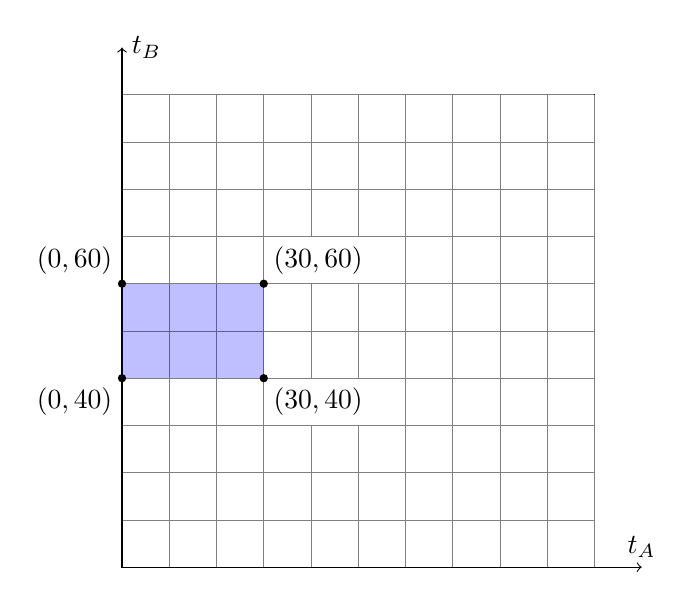
\begin{tikzpicture}[scale=0.6]
    \draw (0,0) rectangle (10,10);
    \draw [help lines] (0,0) grid (10,10);
    \draw [->] (0,0) -- (11,0) node [above] {$t_A$};
    \draw [->] (0,0) -- (0,11) node [right] {$t_B$};
    \fill [nearly transparent, blue] (0,4) -- (0, 6) -- (3,6) -- (3,4);
    \path (0,4) node [below left]  {$(0, 40)$}
          (0,6) node [above left]  {$(0, 60)$}
          (3,6) node [above right, fill=white] {$(30, 60)$}
          (3,4) node [below right, fill=white] {$(30, 40)$};
    \fill (0,4) circle [radius=2.5pt]
          (0,6) circle [radius=2.5pt]
          (3,6) circle [radius=2.5pt]
          (3,4) circle [radius=2.5pt];
  \end{tikzpicture}
\end{center}

\noindent
The blue region depicts the probability $P\{T_A < 30 \cap 40 < T_B < 60\}$. The
probability is equal to the volume of the space underneath it, where the space
is bounded by the probability density function $f$ from the above. Since $f$ is
constant, the volume simply equals to $30 \cdot 20 \cdot \frac{1}{10000} =
\frac{600}{10000} = \frac{3}{50} = 0.06$.

\newpage

\subsection*{c)}

For this question, we must calculate the area of the surface of square with the
constraint $t_A < t_B + 10$.

\begin{center}
  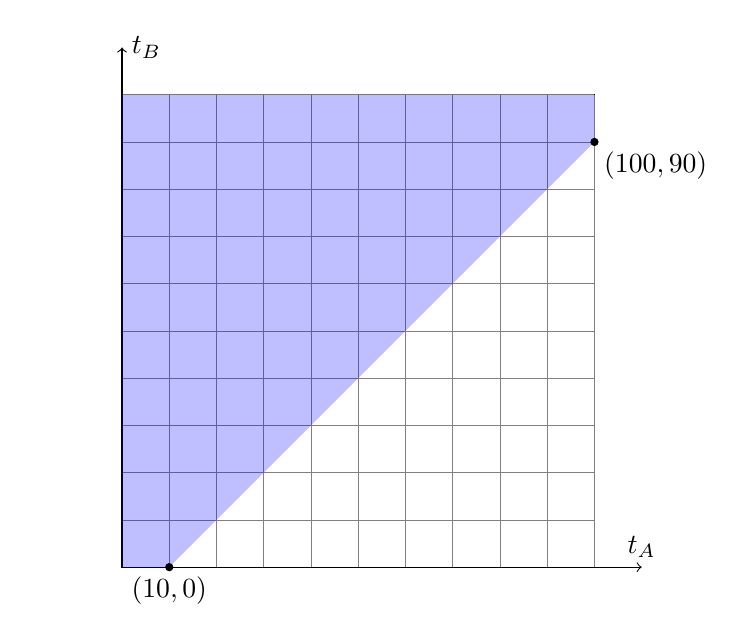
\begin{tikzpicture}[scale=0.6]
    \draw (0,0) rectangle (10,10);
    \draw [help lines] (0,0) grid (10,10);
    \draw [->] (0,0) -- (11,0) node [above] {$t_A$};
    \draw [->] (0,0) -- (0,11) node [right] {$t_B$};
    \fill [nearly transparent, blue]
      (1,0) -- (0,0) -- (0,10) -- (10, 10) -- (10,9) -- (1,0);
    \path (1,0)  node [below] {$(10, 0)$}
          (0,2)  node [transparent, left] {$(0, 20)$}
          (10,9) node [below right] {$(100, 90)$};
    \fill (1,0)  circle [radius=2.5pt]
          (10,9) circle [radius=2.5pt];
  \end{tikzpicture}
\end{center}

\noindent
The area of the surface is $100 \cdot 100 - 90 \cdot 90 \cdot \frac{1}{2} =
5950$. The volume of the space is $5950 \cdot \frac{1}{10000} =
\frac{5950}{10000} = \frac{119}{200} = 0.595$.

\subsection*{d)}

For this question, the inequality $|t_A - t_B| < 20$ must be satisfied. This
equals to $-20 < t_A - t_B < 20$ which means $t_B - 20 < t_A < t_B + 20$.

\begin{center}
  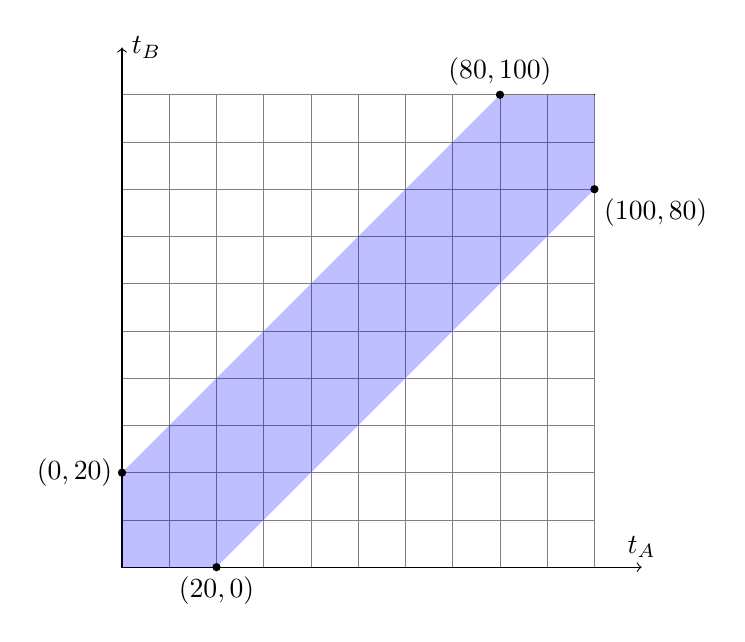
\begin{tikzpicture}[scale=0.6]
    \draw (0,0) rectangle (10,10);
    \draw [help lines] (0,0) grid (10,10);
    \draw [->] (0,0) -- (11,0) node [above] {$t_A$};
    \draw [->] (0,0) -- (0,11) node [right] {$t_B$};
    \fill [nearly transparent, blue]
      (2,0) -- (0,0) -- (0,2) -- (8, 10) -- (10,10) -- (10,8) -- (2,0);
    \path (2,0)  node [below] {$(20, 0)$}
          (0,2)  node [left] {$(0, 20)$}
          (10,8) node [below right] {$(100, 80)$}
          (8,10) node [above] {$(80, 100)$};
    \fill (2,0)  circle [radius=2.5pt]
          (0,2)  circle [radius=2.5pt]
          (10,8) circle [radius=2.5pt]
          (8,10) circle [radius=2.5pt];
  \end{tikzpicture}
\end{center}

\noindent
The area of the surface is $100 \cdot 100 - 2 \cdot 80 \cdot 80 \cdot
\frac{1}{2} = 3600$. The volume of the space is $3600 \cdot \frac{1}{10000} =
\frac{3600}{10000} = \frac{9}{25} = 0.36$.

\newpage

\section*{Answer 2}

\subsection*{a)}

This probability is binomially distributed with parameters $n = 150$, because
150 people are selected from the population, and $p = 0.6$, because frequent
shoppers are $60\%$ of the population. Since $n$ is large, normal approximation
to binomial distribution with parameters $\mu = n \cdot p$ and $\sigma = \sqrt{n
\cdot p \cdot (1 - p)}$ can be used. In that case, $\mu = 90$ and $\sigma = 6$.
In order for the $65\%$ of the customers to be frequent shoppers, at least 97.5
of them should be frequent shoppers.

\begin{align*}
  \boldP\{X > 97.5\}
    &= \boldP \left\{ \frac{X - 90}{6} > \frac{97.5 - 90}{6} \right\} \\
    &=
\end{align*}

\subsection*{b)} 


\section*{Answer 3}


\section*{Answer 4}

\subsection*{a)} 

\subsection*{b)} 

\subsection*{c)} 

\end{document}